% Adapted from Devin-Taylor/TikZ from GitHub (MIT License)
\usetikzlibrary{calc, backgrounds, arrows.meta}

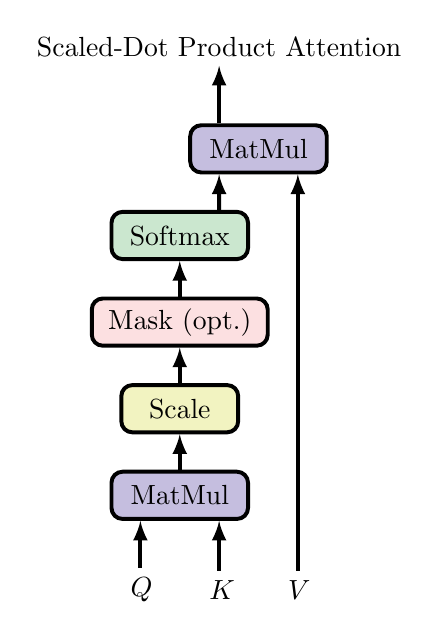
\begin{tikzpicture}[
    >=latex,
]

\definecolor{matmul_color}{RGB}{197,190,223}
\definecolor{emb_color}{RGB}{252,224,225}
\definecolor{add_norm_color}{RGB}{242,243,193}
\definecolor{softmax_color}{RGB}{203,231,207}

\tikzstyle{sqr} = [rectangle, rounded corners, minimum width=1cm, text width=1.25cm, minimum height=.6cm,text centered, draw=black, line width=.5mm]

\node (Q) [text width=.25cm] {$Q$};
\node (K) [text width=.25cm, right of=Q] {$K$};
\node (V) [text width=.25cm, right of=K] {$V$};

\node (matmul) [sqr, fill=matmul_color, above of=K, xshift=-0.5cm, text width=1.5cm, yshift=0.2cm] {MatMul};
\node (scale) [sqr, fill=add_norm_color, above of=matmul, yshift=0.1cm] {Scale};
\node (mask) [sqr, fill=emb_color, above of=scale, yshift=0.1cm, text width=2cm] {Mask (opt.)};
\node (softmax) [sqr, fill=softmax_color, above of=mask, yshift=0.1cm, text width=1.5cm] {Softmax};

\node (matmul2) [sqr, fill=matmul_color, above of=softmax, yshift=0.1cm, xshift=1cm, text width=1.5cm] {MatMul};
\node (scaleddot) [above of=matmul2, yshift=.3cm, xshift=-0.5cm] {Scaled-Dot Product Attention};

\draw[->, line width=.5mm] (matmul.north) -- (scale.south);
\draw[->, line width=.5mm] (scale.north) -- (mask.south);
\draw[->, line width=.5mm] (mask.north) -- (softmax.south);
\draw[->, line width=.5mm] ($ (softmax.north) + (0.5, 0) $) -- ($ (matmul2.south) + (-0.5, 0) $);

\draw[->, line width=.5mm] (Q) -- ($ (matmul.south) + (-0.5, 0) $);
\draw[->, line width=.5mm] (K) -- ($ (matmul.south) + (0.5, 0) $);
\draw[->, line width=.5mm] (V) -- ($ (matmul2.south) + (0.5, 0) $);

\draw[->, line width=.5mm] ($ (matmul2.north) + (-0.5, 0) $) -- (scaleddot.south);

\end{tikzpicture}
